\section{2026년 3월 4일, 18시 42분, 맑음}
안녕 프레키야. 벌써 하루가 지나고 너와 떨어진지는 이틀이 지났구나. 아빠한텐 연락이 오지 않았고, 대신 네 언니한테서 연락이 왔어. 
집에 못 들어온다면 자주 전화해달라면서. 집사는 전화를 걸었고 네 언니가 울음을 참는 소리를 듣고 그 감정을 눈치챘지만 만약 우냐고 물어보면 언니와 집사 모두 
충격 받을 것 같아서 모른채 했어. 그래도 심란한데 동생 목소리 들으니까 조금은 마음이 풀리더라.

사실 아직도 마음이 많이 심란해. 분명 네 첫 생일이 되는 4월 21일 전 주의 토요일에 집에 가서 고양이 케이크도 사주고 첫 생일을 축하해주려 했는데, 
너를 언제 다시 만날지가 기약 없는 기다림이 되어서 지금 많이 무서워. 그 사이에 네가 집사를 잊어버리면 어쩌지, 다시 만났을 때 이틀 전 모습보다 많이 달라져 있으면 어쩌지,
다시 너를 만나지 못하게 되면 어쩌지... 같은 고민을 많이 했고, 이걸 쓰고 있는 지금도 그런 걱정을 하면서 쓰고 있어. 그래도 방금 네 언니가 보내준 사진이랑 영상을 보니 
여전히 아주 쌩쌩하고 귀엽더라ㅋㅋ. 조금은 안심이 되었다고 해야 할까?

어제 고민은 조금 정리했어. 자퇴는 하지 않을거야. 지금까지 쌓아 올린 학업을 포기하는건 너무 아깝고, 무엇보다 3년의 학교 생활을 위해 집사가 노력한게 너무 많아서,
그걸 포기하는건 너무 아쉽단다. 그리고 무엇보다 대학을 나와서 졸업해야 좋은 직장이든 나쁜 직장이든 들어가고 돈을 벌어서 네 간식을 사줄 수 있을테니까. 그리고 아빠한테 
용서를 구하진 않을거야. 집사가 잘못한게 아예 없는건 아니지만 아무리 생각해도 기숙사 오기 전에 방 청소를 게을리 했다, 이건 정말 사소한 일이고, 
일을 이 지경까지 오게 한건 아빠의 저의가 있었든 불안정한 요즘 성격이 많이 불안정한 탓이든, 아빠 쪽에서 많은 요소가 작용했다고 생각하거든. 

사실 아직도 집사는 아빠의 행동을 이해하기 힘들단다. 집사는 지금까지 많은 부분에서 아빠한테 맞춰서 생활했거든. 지금까지 아빠한테 정면으로 대든 적도 없고, 
사춘기 때도 반항하지도 않았고, 고등학교 때 자퇴하겠다고 집사가 울면서 부모한테 하소연한 적이 있었는데, 조금만 더 참자고 해서 고등학교도 무사히 졸업하고, 
원하는대로 국립대에 진학하고, 지금까지 학교를 다니면서 한 학기 놓친거 빼고 장학금도 매 학기 꼬박꼬박 받아서 최대한 부담 안되게 하려 했는데\dots 
부모들은 자식이 8-9를 잘해도 1-2의 못함이 더 신경 쓰이는걸까? 그게 맞다면 부모란 참 이해하기 힘든 존재구나 싶어. 

그리고 뭐 원래도 용돈 같은걸 못 받기도 헀지만 이제 진짜 용돈은 커녕 생활비도 못 받게 되어서 좀 크몽에 넣은 외주를 열심히 홍보해보기로 했어. 아직 들어온 
외주는 하나도 없어서 좀 불안하지만, 한 번쯤은 들어오지 않을까? 사실 외주 하나만 들어와도 금전적으로는 걱정을 좀 덜하게 될 것 같아. 그리고 집사 전자책도 써보려고. 
한 3권 쓴 다음에 전자책 출간 사이트에 난사해보면 한 곳쯤은 받아주겠지. 그 마저도 안된다면 예전처럼 쿠팡에서 알바하면 되니까, 뭐... 모르겠네, 어떻게 될지. 고모들한테 
이 사실을 알려야 하나? 매번 친척들에게 용돈 받는 일로 연락해서 많이 미안하지만, 지금 상황이 그걸 따질 정도로 녹록치 않게 되었으니, 이번 학기는 해야 한다면 
얼굴에 철판 제대로 깔아야 할 것 같아.  

어제 집 분위기가 많이 안 좋았다면 집사가 사과할게. 집사 잘못이 아예 없던건 아니니까. 언니가 말하기를 어제 아빠가 화가 많이 났다면서? 오늘은 괜찮다고 하니 다행이구나. 
하지만 언제 아빠가 집사한테 연락해서 사과든 뭐든 이야기를 하게 될지 모르겠어. 사실 집사도 지금 아빠가 정말 원망스럽고 밉고, 분노스럽고, 
이번 학기가 끝난 후 앞으로의 삶이 두려워. 이젠 무슨 일이 생겨도 돌아갈 집도 없고, 의지할 사람도 없어졌으니. 그리고 이 감정이 언제 끝날지 모르겠어. 차라리 연락해서 욕이라도 했으면 
좋겠다는 생각을 했어. 그럼 집사도 마음 깊이 숨겨놨던 설움이나 감정을 이야기 했을테니까. 언제쯤 연락이 올까. 이 상황이 누군가한텐 심각한 일이라는걸 인지는 
하고 있는걸까? 
지금 당장의 상황이 참 막막하고 마음은 먹먹할 뿐이야. 하지만 프레키 너와 네 언니이자 집사의 여동생인 예은이한텐 악감정이 전혀 없단다. 
오히려 너희 둘을 만나러야 당장 기차를 타고 부산으로 가서 보고 싶어. 너무 보고 싶어. 
사실 하루가 지났지만 너와 동생을 생각하며 이걸 쓰니 다시 또 눈물이 나오는구나. 하지만 어제도 말했듯이 너를 다시 보기 위해 집사는 당장을 참고 꼭 버틸거란다. 
아무리 늦어도 집사가 군대에서 나오는 2년 뒤에는 너를 다시 볼 수 있으리란 희망을 가지며. 쓰고 나니까 너한테 한탄하는 글이 되어버렸네, 이런.

조만간 다시 만나 장난감을 흔들면 채터링하고 잡으려고 소파 위를 방방 뛰어다니던 네 모습을 다시 보고 싶어. 
아 맞다, 그리고 휴대폰에 있는 네 사진이랑 영상들을 Google Drive로 옮기려고 해. 네 사진만 20GB가 넘어가서 얼마나 걸릴진 모르겠지만 
집사 휴대폰이 맛이 가기 일보 직전이라 말이야. 

\bigskip
너를 매일 쓰다듬어 주던 사랑하는 집사 김동준이 대전에서. 사랑을 담아.

\begin{figure}[htbp]
  \centering
  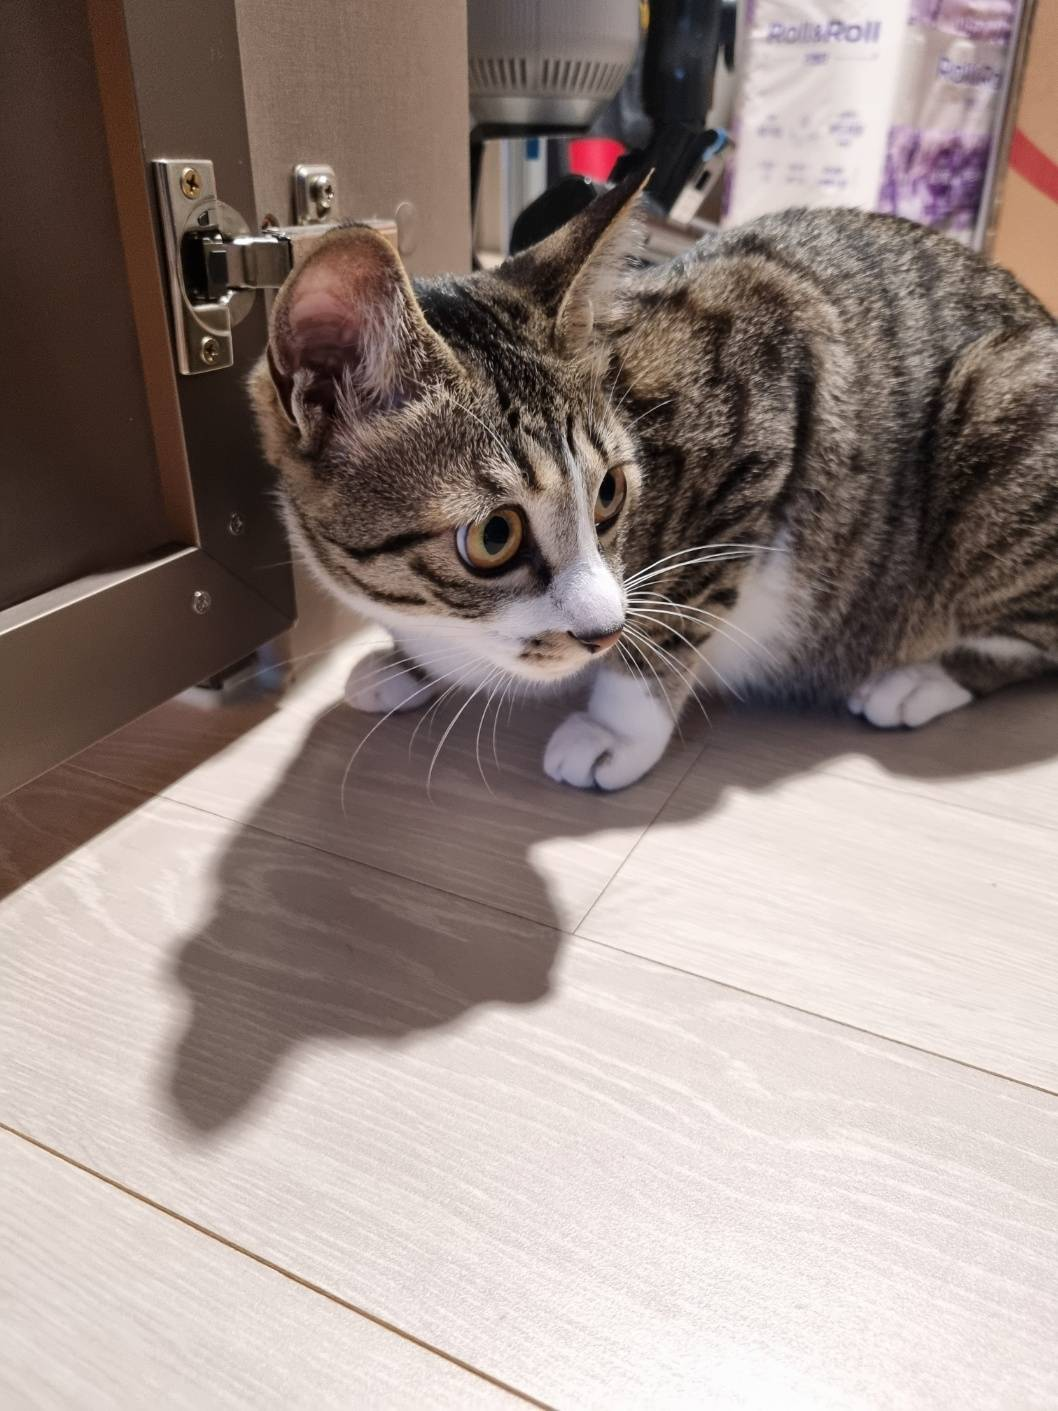
\includegraphics[width=0.38\linewidth]{photo/2026-3-4_0.jpg}\quad
  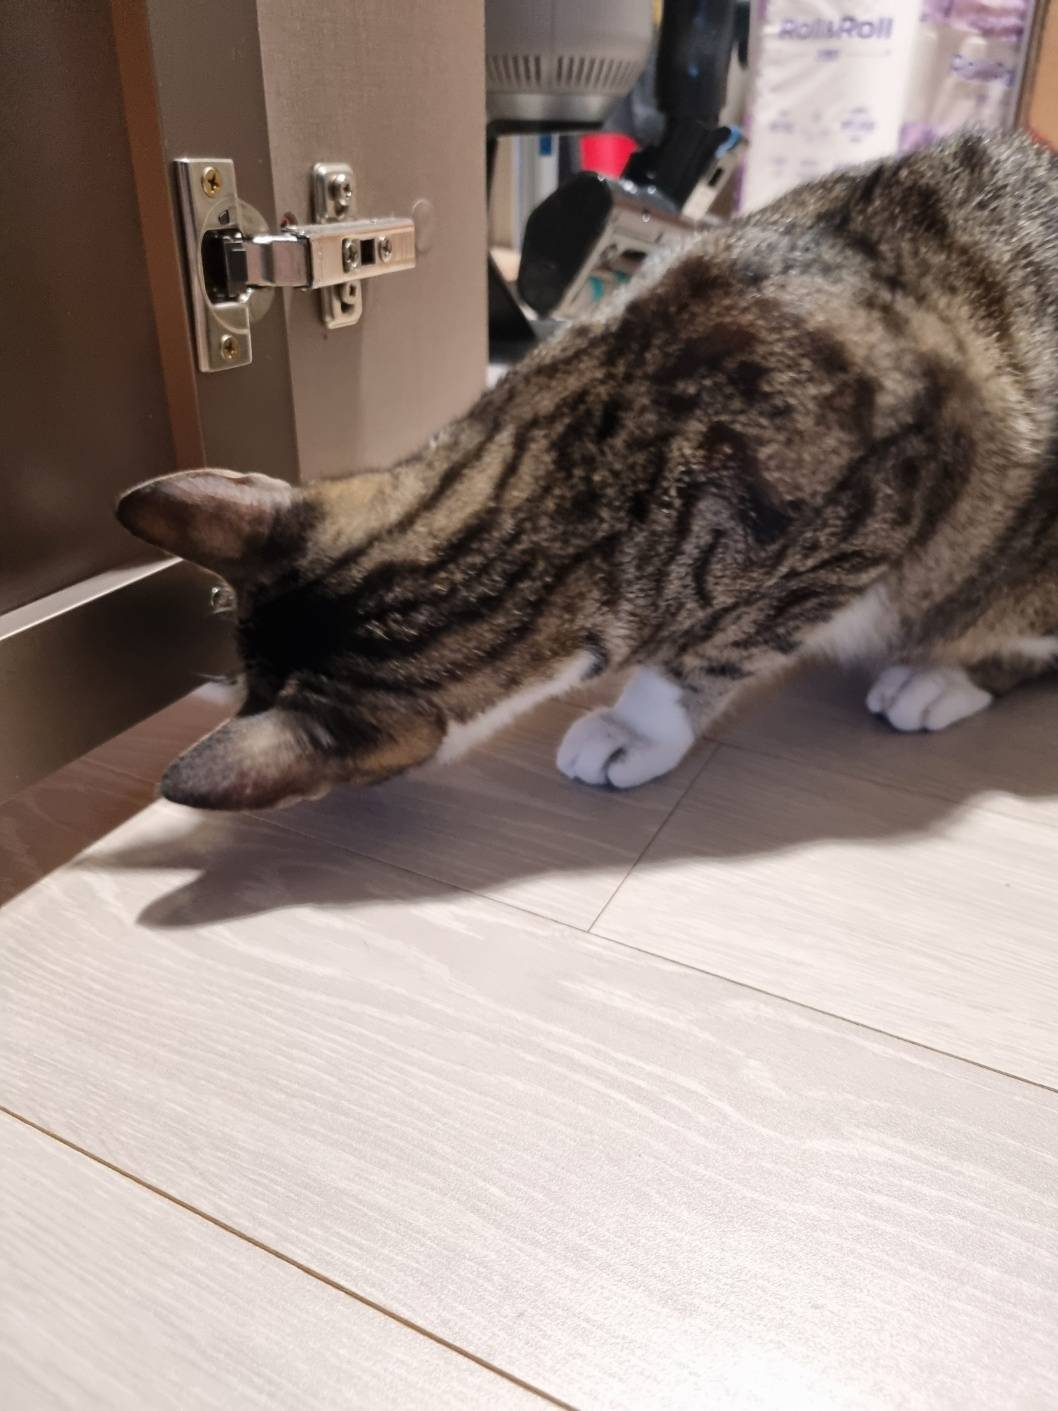
\includegraphics[width=0.38\linewidth]{photo/2026-3-4_1.jpg}\\[10pt]
  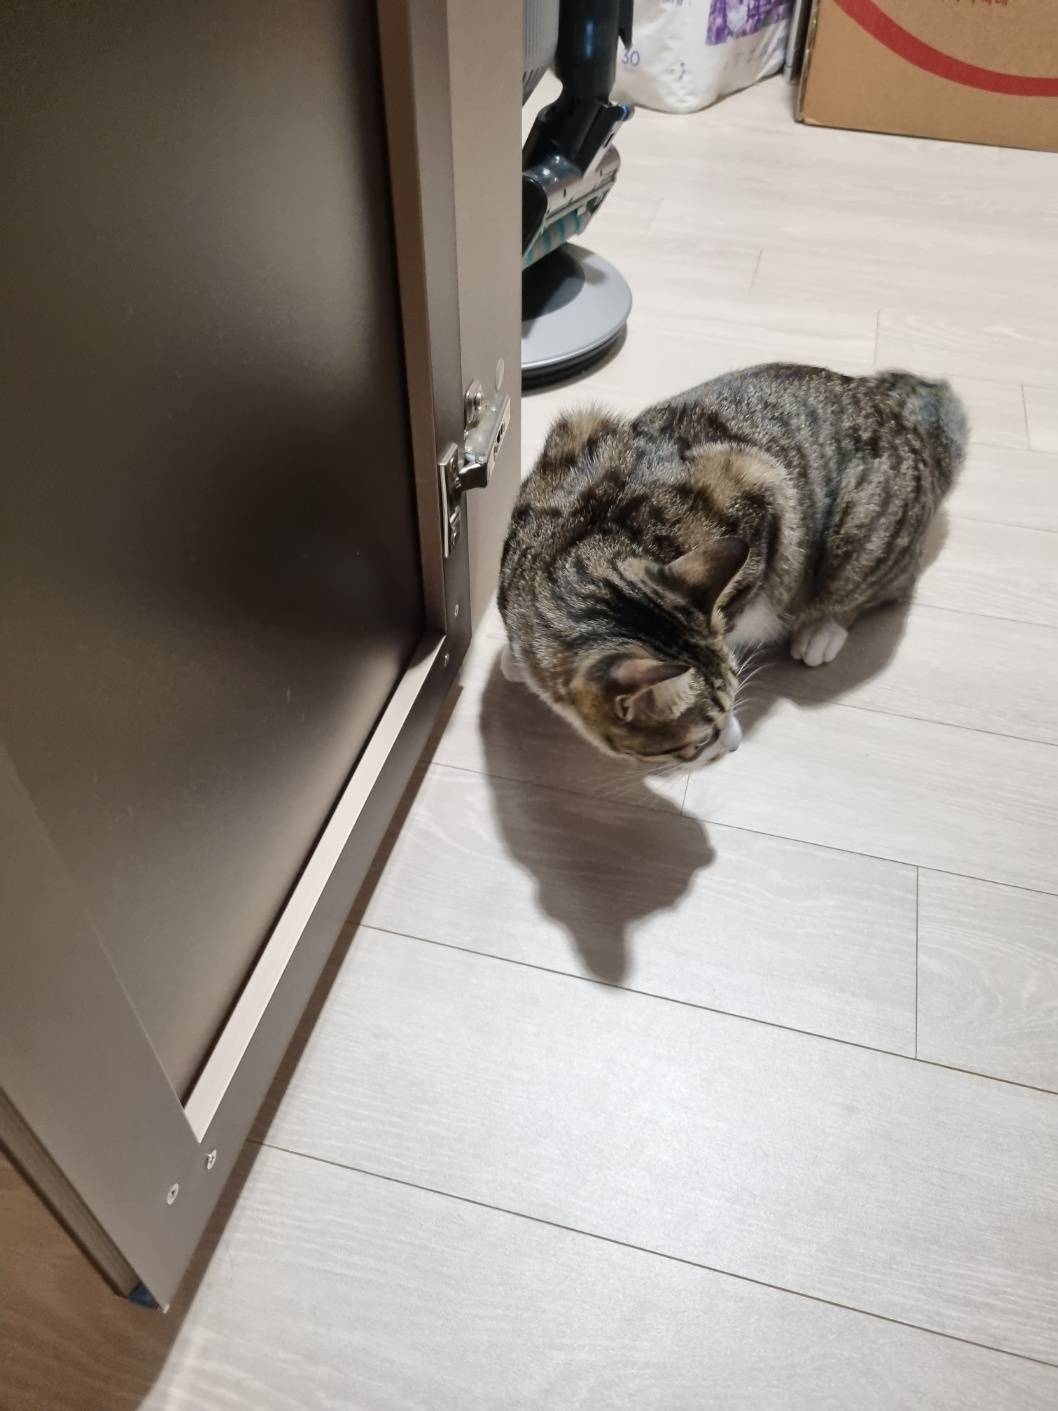
\includegraphics[width=0.38\linewidth]{photo/2026-3-4_2.jpg}\quad
  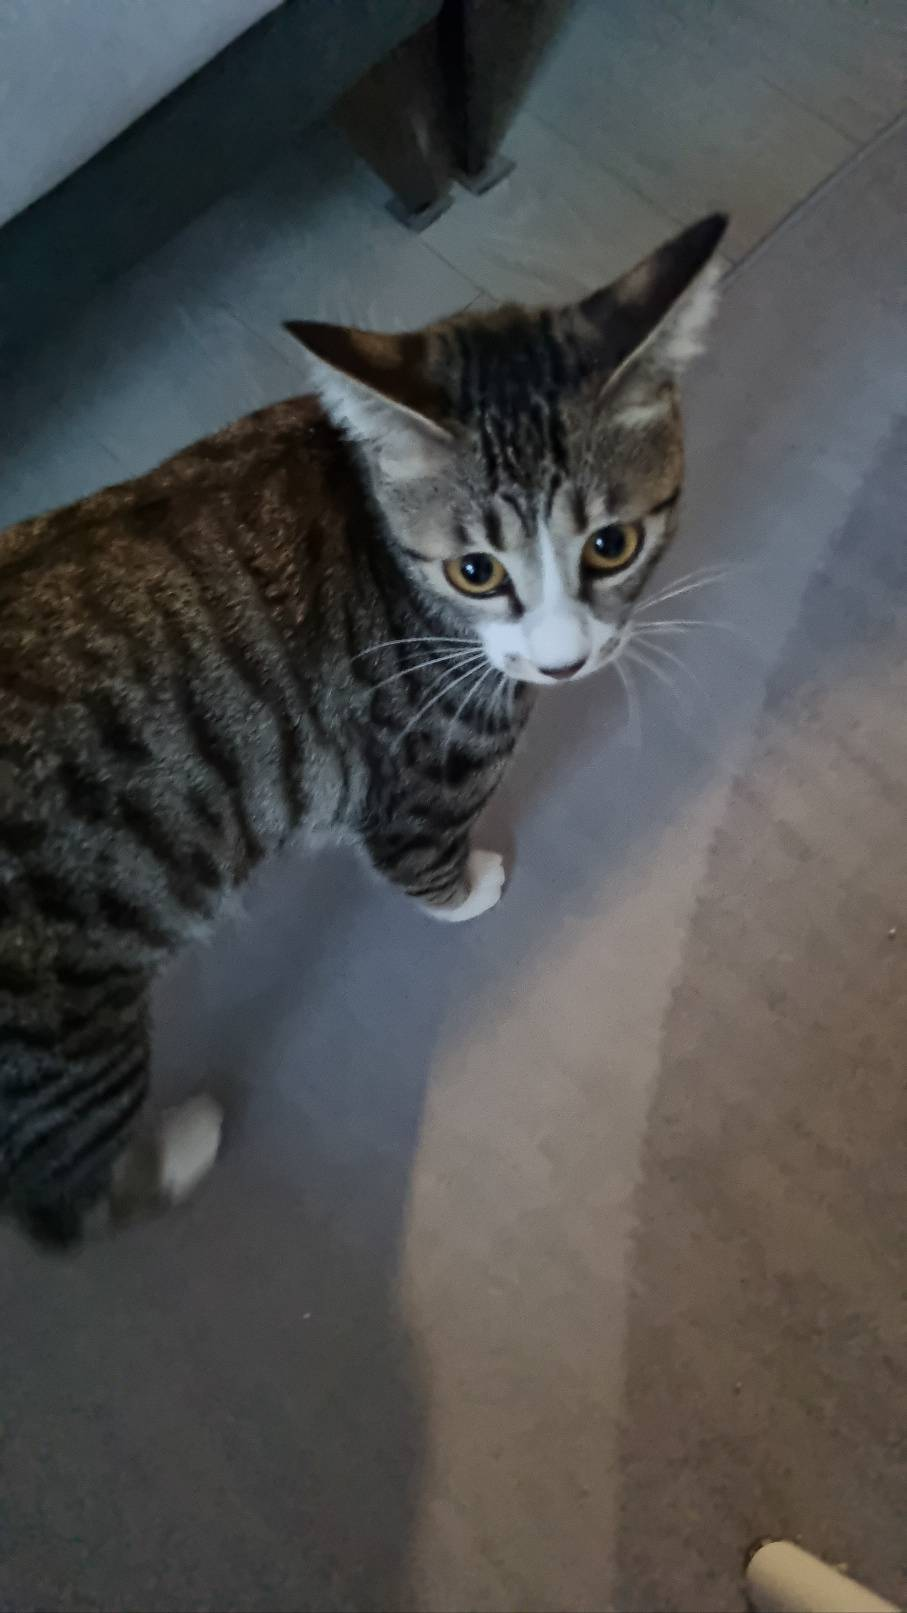
\includegraphics[width=0.38\linewidth]{photo/2026-3-4_3.jpg}
  \caption{오늘 네 언니가 보내준 사진이야. 여전히 너무 귀여워!!!!!}
  \label{fig:2026-3-4}
\end{figure}

\newpage